\documentclass[11pt,a4paper]{article}

\usepackage[margin=2.5cm]{geometry}
\usepackage{amsmath}
\usepackage{graphicx}
\usepackage{booktabs}
\usepackage{siunitx}
\usepackage{hyperref}
\usepackage{natbib}
\usepackage{xcolor}

\title{Stereo-Aware Audio Signal Processing for Speech-Oriented Analysis}
\author{Mubarik Jamal Muuse}
\date{\today}

\begin{document}
\maketitle

\begin{abstract}
This report presents a browser-based audio analysis system with a Python signal-processing backend. The technical focus is not the dashboard itself, but exported quantitative measurement of how preprocessing changes speech-oriented audio features. A verified Harvard speech export, \texttt{harvard.wav}, is used for filter and speech-feature evaluation. A separate LEFT\_RIGHT stereo test clip is used only for stereo diagnostics and channel-analysis evidence. The evaluated pipeline covers sampling, stereo reduction, RMS/dB energy, STFT-based spectral features, mel/MFCC representations, pitch/F0 and VAD-related outputs, high-pass, low-pass and band-pass filtering, pre-emphasis, RMS normalization, spectral noise suppression, and processing-time measurement.
\end{abstract}

\section{Introduction}

Speech and conversational audio are rarely clean mono signals. Recordings may contain unequal stereo channels, low-frequency rumble, high-frequency noise, silence and non-stationary speech events. Before speech activity or prosody can be interpreted, the signal must be converted into documented exported measurements: energy, spectrum, voicing, activity and timing.

The project problem is therefore a signal-processing problem: quantify how channel selection and preprocessing alter measurable audio features. The dashboard is the experimental interface for upload, playback, channel selection and export. The authoritative results are the backend CSV/JSON exports.

Two result sets are used. The speech/filter evaluation uses \texttt{results/filter\_experiment\_mixdown\_speech\_harvard.csv/json}, whose JSON filename is \texttt{harvard.wav}. Stereo analysis uses \texttt{results/filter\_experiment\_mixdown\_stereo\_lrtest.csv/json}, whose source is a LEFT\_RIGHT stereo test clip. This separation is important: speech-like and voiced-frame outputs are interpreted only for the Harvard speech export, while the LEFT\_RIGHT clip is used only to show stereo separation, correlation and mid/side behaviour.

\section{Signal-Processing Method}

\subsection{Sampling and Stereo}

The backend standardizes analysis to $f_s=\SI{16000}{Hz}$, giving a Nyquist limit of \SI{8000}{Hz}. Features are computed from \SI{20}{ms} frames ($320$ samples), exported at \SI{10}{Hz}, and summarized over a \SI{1.0}{s} rolling analysis window. This makes the exports comparable across filter conditions instead of depending on browser playback state.

Stereo is treated as part of the signal, not as a display option. The Harvard speech export is analysed in mixdown mode. The LEFT\_RIGHT stereo clip is used to inspect whether the two channels contain different information. For left and right channels $L[n]$ and $R[n]$, the main reductions are
\begin{align}
    x_{\mathrm{mix}}[n] &= \frac{L[n]+R[n]}{2}, &
    x_{\mathrm{mid}}[n] &= \frac{L[n]+R[n]}{2}, &
    x_{\mathrm{side}}[n] &= \frac{L[n]-R[n]}{2}.
\end{align}
The exported stereo diagnostics report left/right RMS, left-minus-right balance, left-right correlation, mid RMS, side RMS and stereo width. These values show whether mixdown is harmless or whether side-channel information is significant.

\subsection{Frame Features}

RMS and dB measure signal level. RMS is useful because it gives a single energy value for each waveform or condition:
\begin{equation}
    \mathrm{RMS}(x) = \sqrt{\frac{1}{N}\sum_{n=0}^{N-1}x[n]^2},
\end{equation}
and the report converts it to a digital dB value,
\begin{equation}
    E_{\mathrm{dB}} = 20\log_{10}(\mathrm{RMS}(x)+\epsilon).
\end{equation}
This is not calibrated SPL; it is a within-system digital level for comparing preprocessing conditions.

Spectral features measure where energy lies in frequency. The backend uses a Hann-window STFT with FFT size $N_{\mathrm{FFT}}=512$, hop length $H=160$ samples, and window length $400$ samples:
\begin{equation}
    X[m,k] = \sum_{n=0}^{N_{\mathrm{FFT}}-1} x[n+mH]w[n]e^{-j2\pi kn/N_{\mathrm{FFT}}}.
\end{equation}
At \SI{16000}{Hz}, the bin spacing is \SI{31.25}{Hz}. The exported centroid indicates whether energy is concentrated lower or higher in the spectrum; rolloff, computed at 85\% accumulated spectral power, gives a high-frequency spread indicator; flatness separates tonal/structured spectra from noise-like spectra; flux measures frame-to-frame spectral change; and zero-crossing rate increases when the waveform contains more rapid sign changes. These appear directly in the Harvard filter-result tables.

The exported low, speech and high ratios summarize energy below \SI{80}{Hz}, between \SI{80}{Hz} and \SI{4000}{Hz}, and above \SI{4000}{Hz}. These are backend-defined analysis bands. They are useful for this project because the filters use the same boundaries, so the tables can directly show whether high-pass, low-pass and band-pass processing removed the intended frequency regions.

Mel spectrograms and MFCCs are included as speech-oriented spectral representations \citep{mcfee2015librosa}. The backend uses 64 mel bands from \SI{50}{Hz} to \SI{8000}{Hz} and computes 13 MFCC coefficients. The final tables emphasize aggregate descriptors rather than MFCC coefficients, while the mel figure is used qualitatively to show non-stationary speech energy.

Pitch/F0 and VAD are used as backend diagnostics. F0 is estimated with WORLD/pyworld DIO followed by StoneMask refinement \citep{morise2016world}. VAD uses an adaptive noise estimate with SNR hysteresis: on threshold 2.5, off threshold 1.8, and \SI{0.20}{s} hangover \citep{ramirez2007voice}. The resulting voiced ratio and speech-like ratio help characterize the export, but they are not accuracy results because no labels or reference F0 track are available.

\subsection{Filters}

The allowed backend analysis filters are \texttt{noise}, \texttt{highpass}, \texttt{lowpass}, \texttt{bandpass}, \texttt{normalize}, and \texttt{preemphasis}. The high-pass, low-pass and band-pass filters are 4th-order Butterworth filters with cutoffs \SI{80}{Hz}, \SI{4000}{Hz}, and \SIrange{80}{4000}{Hz}. Offline analysis applies them with \texttt{scipy.signal.filtfilt}, so the reported aggregate changes are zero-phase forward/backward filtering results \citep{oppenheim1999discrete}. This is important because the results should reflect spectral changes rather than phase delay.

Pre-emphasis boosts high-frequency components before feature extraction:
\begin{equation}
    y[n]=x[n]-\alpha x[n-1],
\end{equation}
with $\alpha=0.97$. It is expected to increase centroid, rolloff, high-band ratio and zero-crossing rate. RMS normalization changes level toward target RMS 0.1 and clips output to $[-1,1]$; it should change RMS more than spectral ratios. Spectral noise suppression estimates a median STFT magnitude profile per frequency bin, keeps bins at least 1.5 times that profile, and reconstructs the signal. Because it is signal-dependent, it has no fixed linear magnitude response.

Processing speed is reported as a diagnostic export rather than a benchmark. The report uses
\begin{equation}
    \mathrm{speed\ factor}=\frac{\mathrm{audio\ duration}}{\mathrm{processing\ time}},
    \qquad
    \mathrm{RTF}=\frac{\mathrm{processing\ time}}{\mathrm{audio\ duration}}.
\end{equation}
Thus speed factor greater than 1 means faster-than-real-time processing, while RTF is its inverse.

\section{Implementation}

The implementation separates playback and analysis. Browser playback filters let the user hear changes immediately. Backend analysis loads the selected clip, applies the selected channel mode and preprocessing condition, computes features, and exports CSV/JSON tables. This separation matters because a playback slider does not change exported metrics until backend processing is run again.

The Harvard speech export has filename \texttt{harvard.wav}, duration \SI{18.35625}{s}, analysis sample rate \SI{16000}{Hz}, channel count 2 and channel mode \texttt{mixdown}. The LEFT\_RIGHT stereo export has filename \texttt{freesound\_community-leftright1648-107900.mp3}, duration \SI{2.592}{s}, analysis sample rate \SI{16000}{Hz}, channel count 2 and channel mode \texttt{side}. Both exports use the same filter cutoffs: \SI{80}{Hz}, \SI{4000}{Hz}, and \SIrange{80}{4000}{Hz}.

The exported feature rows use the fixed backend settings listed above: \SI{16000}{Hz} sample rate, \SI{20}{ms} frames, \SI{10}{Hz} feature output rate, \SI{1.0}{s} rolling window, Hann-window STFT $512/160/400$, rolloff fraction 0.85, 64 mel bands from \SI{50}{Hz} to \SI{8000}{Hz}, 13 MFCC coefficients, pyworld DIO+StoneMask F0, VAD SNR thresholds 2.5/1.8 with \SI{0.20}{s} hangover, 4th-order zero-phase Butterworth filters, pre-emphasis coefficient 0.97, and RMS-normalization target 0.1. These settings are held fixed across filter rows. The exports and code are sufficient for numeric comparison of aggregate features, stereo diagnostics and timing, but not for full validation: the CSV/JSON files still omit original audio source metadata, labelled speech annotations, F0 reference tracks, repeated timing runs, and the hardware/software timing environment.

\section{Experiments and Results}

\subsection{Harvard Speech Filter Experiment}

Table~\ref{tab:harvard-main} reports the verified Harvard speech export. The raw clip has RMS \SI{-25.03}{dB}, centroid \SI{1672.70}{Hz}, and speech-band ratio 0.7945. High-pass filtering at \SI{80}{Hz} reduces the low-band ratio from 0.0484 to 0.00006 and raises centroid to \SI{2028.47}{Hz}. Low-pass filtering at \SI{4000}{Hz} reduces the high-band ratio from 0.1571 to 0.00015 and lowers centroid to \SI{947.40}{Hz}. The band-pass condition suppresses both low and high ratios to approximately zero and concentrates almost all exported band energy in the backend speech band, 0.9998.

\begin{table}[h]
\centering
\caption{Harvard speech filter results from \texttt{filter\_experiment\_mixdown\_speech\_harvard.csv/json}.}
\label{tab:harvard-main}
\small
\begin{tabular}{lrrrrrr}
\toprule
Condition & RMS dB & Centroid Hz & Rolloff Hz & Low & Speech & High \\
\midrule
Raw & -25.03 & 1672.70 & 3086.72 & 0.0484 & 0.7945 & 0.1571 \\
HP 80 Hz & -28.76 & 2028.47 & 3666.19 & 0.0001 & 0.8330 & 0.1669 \\
LP 4000 Hz & -25.14 & 947.40 & 1854.25 & 0.0576 & 0.9423 & 0.0001 \\
BP 80--4000 Hz & -29.00 & 1209.97 & 2215.29 & 0.0001 & 0.9998 & 0.0001 \\
Noise suppression & -25.04 & 1438.86 & 2494.64 & 0.0465 & 0.7958 & 0.1577 \\
RMS normalization & -20.27 & 1672.72 & 3086.62 & 0.0484 & 0.7945 & 0.1571 \\
Pre-emphasis & -34.84 & 3350.83 & 5449.55 & 0.0001 & 0.1281 & 0.8718 \\
\bottomrule
\end{tabular}
\end{table}

Table~\ref{tab:harvard-extra} shows exported descriptors related to timbral change, voicing and speech-like activity. Pre-emphasis has the strongest high-frequency effect: centroid increases by \SI{1678.13}{Hz}, rolloff increases to \SI{5449.55}{Hz}, ZCR increases to 0.3630, and high-band ratio rises to 0.8718. RMS normalization behaves as expected spectrally: centroid, rolloff and band ratios remain essentially unchanged while RMS increases by \SI{4.77}{dB}. Spectral noise suppression changes RMS only by \SI{-0.008}{dB}, lowers centroid by \SI{233.84}{Hz}, and leaves high-band ratio almost unchanged. The voiced and speech-like ratios are reported only as backend diagnostic outputs; no VAD or F0 accuracy is claimed because no speech/non-speech labels or reference F0 track are included.

\begin{table}[h]
\centering
\caption{Additional Harvard descriptors and exported speed factor. Speed factor is audio duration divided by processing time; real-time factor is the inverse, processing time divided by audio duration.}
\label{tab:harvard-extra}
\small
\begin{tabular}{lrrrrr}
\toprule
Condition & Flatness & Flux & ZCR & Voiced & Speed factor \\
\midrule
Raw & 0.0514 & 3.0341 & 0.1321 & 0.9185 & 2.230 \\
HP 80 Hz & 0.0729 & 2.0674 & 0.1873 & 0.9511 & 2.072 \\
LP 4000 Hz & 0.0141 & 2.8213 & 0.0763 & 0.9185 & 2.158 \\
BP 80--4000 Hz & 0.0141 & 1.8192 & 0.1180 & 0.9457 & 2.064 \\
Noise suppression & 0.1085 & 2.9869 & 0.1161 & 0.9185 & 2.151 \\
RMS normalization & 0.0498 & 5.3379 & 0.1321 & 0.9185 & 2.153 \\
Pre-emphasis & 0.1383 & 1.1988 & 0.3630 & 0.9185 & 2.214 \\
\bottomrule
\end{tabular}
\end{table}

All Harvard conditions run faster than real time in this single exported diagnostic run. Processing times range from \SI{8.232}{s} for raw analysis to \SI{8.892}{s} for band-pass processing; the corresponding speed factors are 2.230 and 2.064, so their real-time factors are the inverses, approximately 0.448 and 0.484. The JSON reports total experiment processing time \SI{59.880}{s}. These timings are not benchmark-level performance claims because the export does not include hardware, software versions, repeated runs, or whether decoding and I/O are included.

\subsection{Figures}

Figure~\ref{fig:spectrum} shows the exported before/after spectrum comparison over the 0--\SI{8000}{Hz} analysis range. It is consistent with the table-based interpretation that preprocessing changes spectral distribution, especially centroid and rolloff. However, because the image does not encode the selected filter state or dB reference, the numeric centroid, rolloff and band-ratio values in Tables~\ref{tab:harvard-main}--\ref{tab:harvard-extra} remain the authoritative evidence.

\begin{figure}[h]
\centering
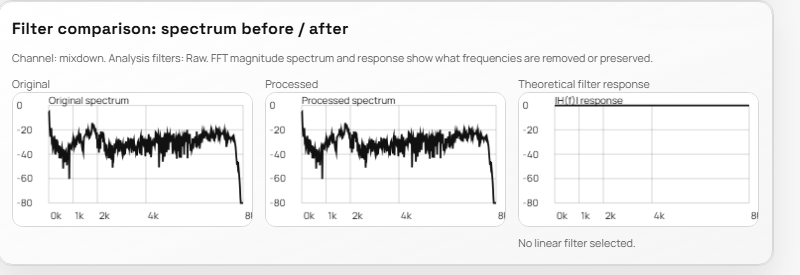
\includegraphics[width=0.78\linewidth]{figures/HARVARD_filter_comparison_spectrum_before_after.png}
\caption{Exported before/after spectrum comparison. The figure supports the qualitative direction of spectral redistribution, but the numeric evidence remains Tables~\ref{tab:harvard-main}--\ref{tab:harvard-extra} because the PNG does not encode the selected filter state or dB reference.}
\label{fig:spectrum}
\end{figure}

Figure~\ref{fig:mel} shows the saved Harvard mel spectrogram. The alternating dark and high-energy vertical regions show that the clip is non-stationary, as expected for speech with pauses and syllabic energy changes. The stronger energy in lower and mid mel bands is consistent with the raw export having most energy in the backend speech band. The figure is still qualitative because the PNG does not store the exact plotting scale.

\begin{figure}[h]
\centering
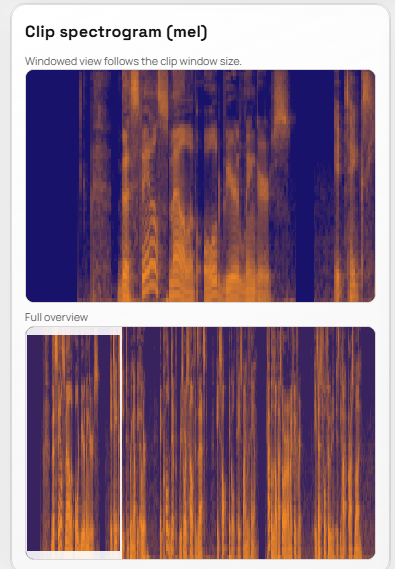
\includegraphics[width=0.55\linewidth]{figures/HARVARD_speech_harvard_mel_spectrogram.png}
\caption{Exported Harvard mel spectrogram. The figure supports the claim that the speech clip is non-stationary with stronger low/mid-band energy, but it is not used for quantitative measurement because the saved PNG does not encode the plotting scale.}
\label{fig:mel}
\end{figure}

\subsection{LEFT\_RIGHT Stereo Diagnostics}

The LEFT\_RIGHT stereo clip is used only for stereo/channel analysis. Table~\ref{tab:stereo} shows that the left and right channel levels are nearly balanced: the right channel is only \SI{0.04}{dB} higher than the left. The left-right correlation is approximately zero ($-0.000007$), so the recording is not dual mono. Mid RMS and side RMS are both \SI{-33.63}{dB}, and stereo width is 0.5000. This supports the report's claim that channel mode is a real signal-processing choice: the left and right spectra differ strongly, and the non-zero side channel contains meaningful stereo information.

\begin{table}[h]
\centering
\caption{LEFT\_RIGHT stereo diagnostics from \texttt{filter\_experiment\_mixdown\_stereo\_lrtest.json}.}
\label{tab:stereo}
\begin{tabular}{lr}
\toprule
Diagnostic & Value \\
\midrule
Left RMS dB & -30.64 \\
Right RMS dB & -30.59 \\
Balance, left minus right dB & -0.04 \\
Left-right correlation & -0.000007 \\
Mid RMS dB & -33.63 \\
Side RMS dB & -33.63 \\
Stereo width & 0.5000 \\
\bottomrule
\end{tabular}
\end{table}

Figure~\ref{fig:stereo} shows the exported left, right, mid and side spectra. The left and right spectra differ strongly, and the side spectrum remains substantial. This agrees with the numeric result: the channels are nearly uncorrelated, and the side channel contains meaningful stereo information.

\begin{figure}[h]
\centering
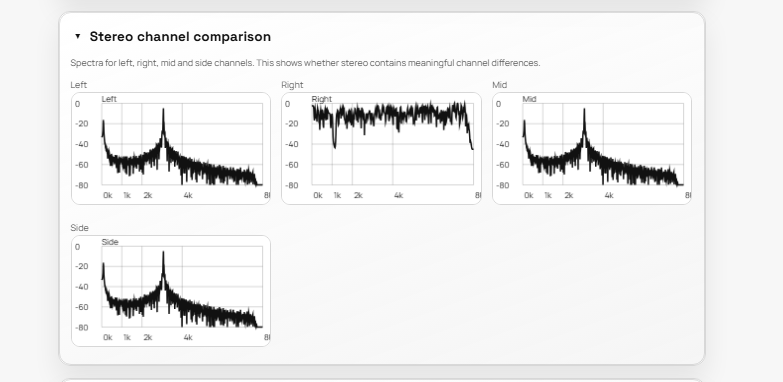
\includegraphics[width=0.90\linewidth]{figures/LEFT_RIGHT_stereo_channel_comparison_lrtest.png}
\caption{Exported stereo channel comparison for the LEFT\_RIGHT stereo clip. The figure supports the mid/side interpretation in Table~\ref{tab:stereo}, but the stereo evidence remains diagnostic because the main exported feature table is for the selected side channel rather than separate left/right/mid/side rows.}
\label{fig:stereo}
\end{figure}

\section{Discussion and Limitations}

The Harvard results show the expected direction for the main filters. High-pass removes low-band energy and raises centroid. Low-pass removes high-band energy and lowers centroid and rolloff. Band-pass concentrates the exported band energy in the speech band. RMS normalization changes level with minimal spectral-ratio change. Pre-emphasis strongly increases high-frequency dominance, shown by centroid, rolloff, high-band ratio and ZCR.

The strongest remaining limitation is validation rather than parameter reporting. The report identifies the main backend settings used for spectral features, F0/VAD outputs and filters, but the exports still do not contain labelled speech annotations, F0 reference tracks, original recording metadata, or repeated timing measurements. For that reason, VAD, speech-like and voiced-frame ratios are reported as backend diagnostic outputs, not validated speech-activity or pitch results.

The figures strengthen the report but are not complete experimental evidence. The Harvard spectrum and mel images lack explicit exported axes and scaling parameters. The LEFT\_RIGHT appendix contains an illustrative narrow band-pass response, but it is not the authoritative Harvard \SIrange{80}{4000}{Hz} result because the shown passband differs from the main experiment. There is also no waveform, VAD overlay or F0 track. The stereo figure is useful qualitatively, but no CSV/JSON export gives separate left, right, mid and side feature rows.

\section{Conclusion}

The project demonstrates a stereo-aware speech-oriented audio analysis pipeline with exported quantitative measurements. On \texttt{harvard.wav}, the filter experiment gives coherent numerical changes for high-pass, low-pass, band-pass, normalization and pre-emphasis. On the LEFT\_RIGHT stereo clip, stereo diagnostics show near-zero channel correlation and substantial side-channel energy. The system is therefore best understood as a signal-processing dashboard with exported quantitative measurements, not merely an interface. To reach a stronger final standard, the backend should add validation figures and labels, especially matched filter responses, VAD overlays and F0 tracks.

\appendix
\section{Data and Export Files}

Speech/filter experiment: \texttt{harvard.wav}, exported as \texttt{results/filter\_experiment\_mixdown\_speech\_harvard.json} and \texttt{results/filter\_experiment\_mixdown\_speech\_harvard.csv}.

Stereo diagnostics: LEFT\_RIGHT stereo clip \texttt{freesound\_community-leftright1648-107900.mp3}, exported as \texttt{results/filter\_experiment\_mixdown\_stereo\_lrtest.json} and \texttt{results/filter\_experiment\_mixdown\_stereo\_lrtest.csv}.

\section{Additional Dashboard Evidence}

Figure~\ref{fig:appendix-bandpass-response} is an illustrative dashboard screenshot of a narrow band-pass response. It demonstrates how an aggressive band-pass can remove most spectral content outside its selected passband, but it is not used as the authoritative Harvard \SIrange{80}{4000}{Hz} filter result.

\begin{figure}[h]
\centering
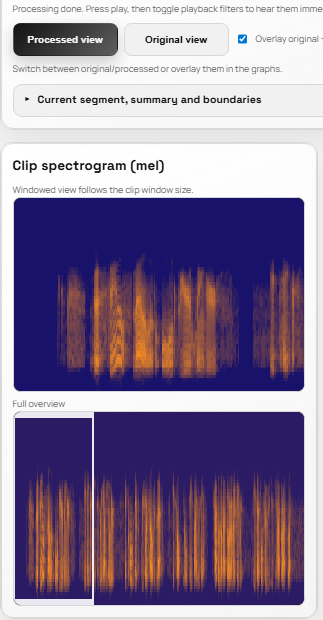
\includegraphics[width=0.82\linewidth]{figures/LEFT_RIGHT_filter_response_bandpass_demo.png}
\caption{Illustrative LEFT\_RIGHT dashboard band-pass response. This supports the qualitative idea of passband-limited filtering, but it is not the quantitative Harvard filter experiment.}
\label{fig:appendix-bandpass-response}
\end{figure}

Figures~\ref{fig:appendix-mel-original}--\ref{fig:appendix-mel-processed} are appendix examples of before/after mel-spectrogram views from the LEFT\_RIGHT dashboard evidence. They visually demonstrate that band-pass filtering reduces the visible mel-spectral region, but they are not used as the main quantitative Harvard result because they come from the LEFT\_RIGHT demonstration and may use different filter settings.

\begin{figure}[h]
\centering
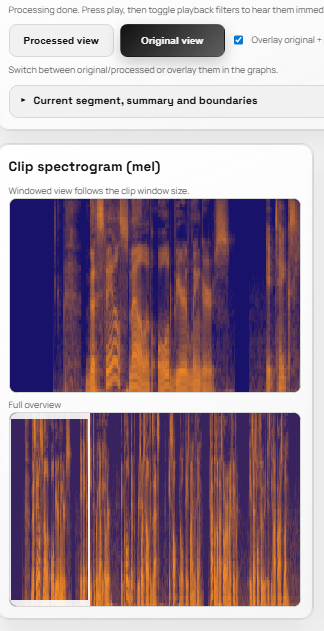
\includegraphics[width=0.62\linewidth]{figures/LEFT_RIGHT_speech_original_mel.png}
\caption{Illustrative LEFT\_RIGHT original mel spectrogram before the dashboard band-pass demonstration.}
\label{fig:appendix-mel-original}
\end{figure}

\begin{figure}[h]
\centering
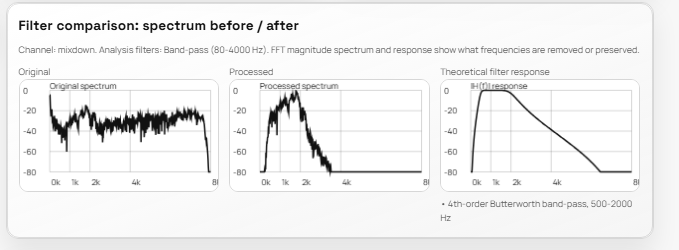
\includegraphics[width=0.62\linewidth]{figures/LEFT_RIGHT_speech_processed_mel_bandpass_demo.png}
\caption{Illustrative LEFT\_RIGHT processed mel spectrogram after the dashboard band-pass demonstration. The reduced visible mel-spectral region supports the qualitative effect of narrow band-pass filtering, not the quantitative Harvard results.}
\label{fig:appendix-mel-processed}
\end{figure}

\begin{thebibliography}{9}

\bibitem[McFee et~al.(2015)]{mcfee2015librosa}
McFee, B., Raffel, C., Liang, D., Ellis, D. P. W., McVicar, M., Battenberg, E., and Nieto, O. (2015).
\newblock librosa: Audio and music signal analysis in Python.
\newblock In \emph{Proceedings of the 14th Python in Science Conference}, 18--25.

\bibitem[Morise et~al.(2016)]{morise2016world}
Morise, M., Yokomori, F., and Ozawa, K. (2016).
\newblock WORLD: A vocoder-based high-quality speech synthesis system for real-time applications.
\newblock \emph{IEICE Transactions on Information and Systems}, E99.D(7), 1877--1884.

\bibitem[Oppenheim and Schafer(1999)]{oppenheim1999discrete}
Oppenheim, A. V. and Schafer, R. W. (1999).
\newblock \emph{Discrete-Time Signal Processing}.
\newblock Prentice Hall.

\bibitem[Ram\'irez et~al.(2007)]{ramirez2007voice}
Ram\'irez, J., G\'orriz, J. M., and Segura, J. C. (2007).
\newblock Voice activity detection. Fundamentals and speech recognition system robustness.
\newblock In \emph{Robust Speech Recognition and Understanding}. I-Tech.

\end{thebibliography}

\end{document}
